\documentclass{article}
\usepackage[utf8]{inputenc}
\usepackage{graphicx}
\usepackage{subcaption}
\usepackage[bottom=0.5in,top=0.5in,right=1in,left=1in]{geometry}
\usepackage[section]{placeins}
\usepackage{float}
\title{Experiment 7}
\author{Nitish Kumar Thakur \\ 21531010 }
\date{14 september, 2021}

\begin{document}

\maketitle

\section{Objective}
Design and fabricate a frequency multiplier circuit using PLL IC-565
 
 \section{Components and Equipment Required}                    
 IC-565*IC-7474 *DSO *Power supply (variable)*connecting wire *Breadboard *probes *Resistance*Function generator
 
 
\section{Theory}

\subsection{Phase lock loop}
Phase-locked loop is a feedback control system that automatically adjusts the phase of a locally generated signal to match the phase of an input signal. PLLs operate by producing an oscillator frequency to match the frequency of an input signal. In this locked condition, any slight change in the input signal first appears as a change in phase between the input signal and the oscillator frequency. This phase shift then acts as an error signal to change the frequency of the local PLL oscillator to match the input signal. The locking-onto-a-phase relationship between the input signal and the local oscillator accounts for the name phase-locked loop.
\begin{figure*}[h]
	\centering
	\includegraphics[scale=0.65]{3 (1).png}
	\caption{PLL}
	\label{FBD}
\end{figure*}
if we analyse the figure there is basically 4 Block.
\subsubsection{Phase Detector}
A phase detector is nothing but a comparator.It performs a comparison of two frequency component fed at its input and generates a dc voltage.This generated voltage is proportional to the difference in phase of the two frequencies.

\subsubsection{Low pass filter}
The output of the phase detector is provided to a low pass filter.It eliminates the high-frequency component and noise from the output of the comparator.This low-frequency dc voltage signal is then provided to a dc  amplifier which amplifies the signal level.This amplified signal is then provided to the VCO

\subsubsection{Voltage Controlled Oscillator}
Voltage-controlled oscillator is electronic oscillator the work of VCO is when we give variable voltage in VCO it generates varying frequency curve(Linear).This thing shown in below Figure
The output of LPF acts as a control signal to the VCO.The VCO generates a dc signal, the amplitude of which is  proportional to the amplitude of output of LPF.Here the adjustment in the output frequency of VCO is made until it shows equivalency with the input signal frequency.

\begin{figure*}[h]
	\centering
	\includegraphics[scale=0.8]{22.png}
	\caption{Voltage-controlled oscillator}
	\label{FBD}
\end{figure*}



\subsubsection{Dc Amplifier}
Amount of gain we getting is very-very less so we use DC amplifier.

Phase Lock Loop basically work in two mode \par
1.Capture range\par2.Lock range\par

\textbf{1.Capture range}\par
The process of adjusting the VCO frequency and holding it to incoming signals frequency is called capture.The minimum and maximum input frequencies to which the loop can move the VCO as it captures an input signal is called the capture range.The segments of the capture range above and below fo are called the pull-in range.The pull-in ranges are not necessarily symmetrical.\par
\par

\textbf{2.Lock range} \par
If the input frequency has moved so far that any further change will cause the control signal to move back and the VCO frequency away from the input signal.The loop is no longer locked and the input and VCO frequencies are no longer the same.The range of input frequencies between the value at which the loop is locked is called the loop’s lock range.The lock range above and below f0 are called the loop’s hold ranges.The lock range is not always centered on f0

\begin{figure}[h]
  \begin{subfigure}[b]{0.6\textwidth}
    \includegraphics[width=\textwidth]{10.jpg}
    \caption{Capture range/ Lock range}
    \label{fig:1}
  \end{subfigure}
  %
  \begin{subfigure}[b]{0.45\textwidth}
    \includegraphics[width=\textwidth]{11 (1).png}
    \caption{Free running Frequency of VCO }
    \label{fig:2}
  \end{subfigure}
\end{figure}




\subsection{IC Pin diagram/ block diagram}
\begin{figure}[ht]
  \begin{subfigure}[b]{0.4\textwidth}
    \includegraphics[width=\textwidth]{5 (1).png}
    \caption{ IC LM-565 Pin diagram}
    \label{fig:1}
  \end{subfigure}
  %
  \begin{subfigure}[b]{0.4\textwidth}
    \includegraphics[width=\textwidth]{6.png}
    \caption{Block diagram of IC LM-565}
    \label{fig:2}
  \end{subfigure}
\end{figure}
\begin{figure}[ht]
  \begin{subfigure}[b]{0.3\textwidth}
    \includegraphics[width=\textwidth]{500.png}
    \caption{ IC 7474 Pin diagram}
    \label{fig:1}
  \end{subfigure}
  %
  \begin{subfigure}[b]{0.3\textwidth}
    \includegraphics[width=\textwidth]{2.png}
    \caption{Block diagram of IC 7474}
    \label{fig:2}
  \end{subfigure}
\end{figure}











\subsection{Frequency division }
When we connect D flip flop complement-Q output to input that means D then output Q is mainly divide the frequency of clock f/2 .it is shown in below figure.
\begin{figure*}[ht]
	\centering
	\includegraphics[scale=0.615]{11.png}
	\caption{Frequency division circuit}
	\label{FBD}
\end{figure*}





\subsection{Frequency multiplier circuit}
if we analyse the Block diagram of frequency multiplier,a divide by N network is inserted between the VCO output (pin 4) and the phase comparator input (pin 5). Since the output of the divider is locked to the input frequency fi, the VCO is actually running at a multiple of the input frequency. Therefore, in the locked state, the VCO output frequency fo is given by,



\begin{figure}[h]
  \begin{subfigure}[b]{0.5\textwidth}
    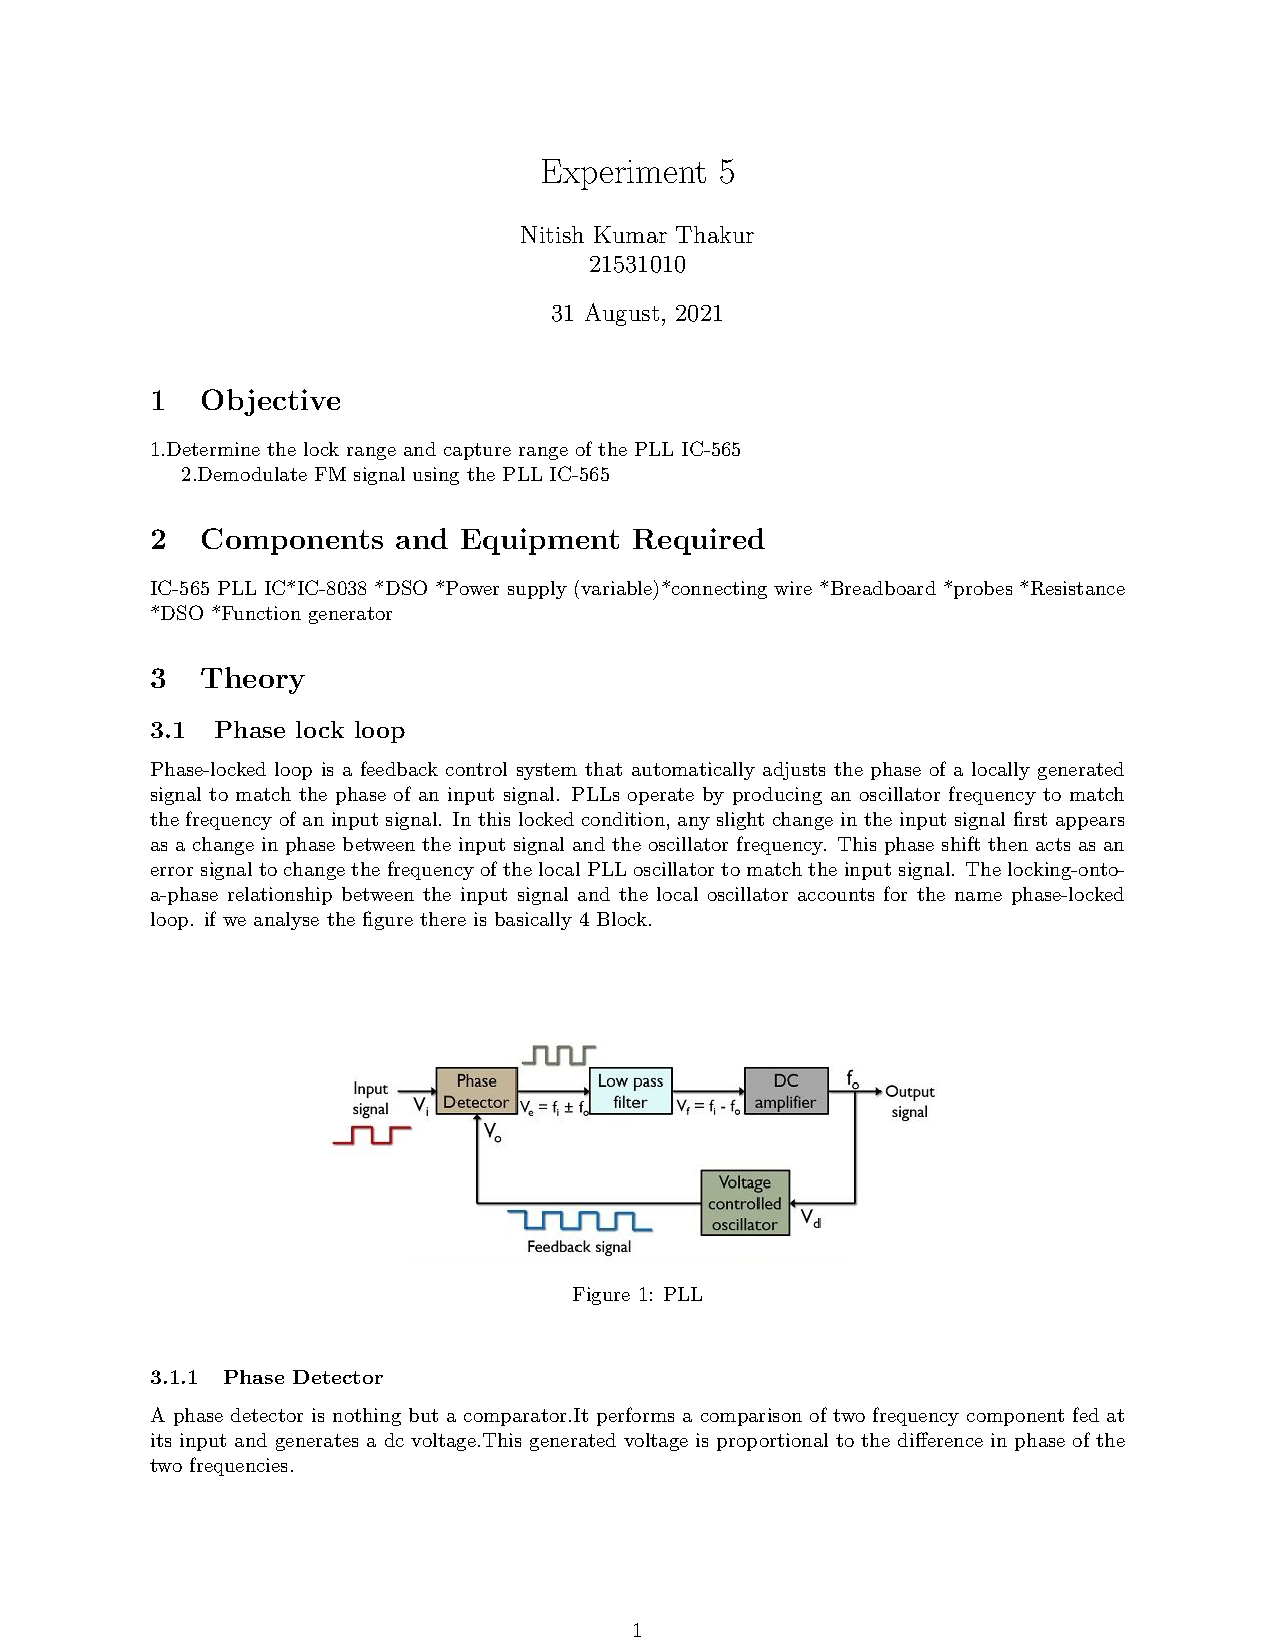
\includegraphics[width=\textwidth]{5.png}
    \caption{ Circuit diagram of freq. multiplier}
    \label{fig:1}
  \end{subfigure}
  %
  \begin{subfigure}[b]{0.5\textwidth}
    \includegraphics[width=\textwidth]{Frequency-Multiplier-using-PLL-565-001.jpg}
    \caption{Block diagram of Frequency multiplier}
    \label{fig:2}
  \end{subfigure}
\end{figure}

















\section{Observation/Results}
When we introduce the frequency divider(IC-7474),in between phase detector and vco,what happens, the frequency from vco divided by N times(f/N).so when these frequency  pass through phase detector it generates some error signal again these signal comeback to  input of VCO,so VCO bump up these signal by N times.so signal even after passing through Divider ckt the frequency matches with phase detector.\par

output of vco-pin4-----pin-3 of IC7474\par
Output of 7474-pin5-----pin-5 of IC865\par


The free running frequency =37Khz \par
At 14 khz it lock the signal after this we increases the signal slowly and see up which point  it lock.,this things happen at Fl2=43Khz;
afte this we decrease the frequency and see from which point again capture the signal,the point is fc2=39Khz,and again slowly we decreases and upto which point it is so fc1=21khz.\par 


\begin{figure*}[ht]
	\centering
	\includegraphics[scale=0.615]{bread.png}
	\caption{Circuit on Breadboard}
	\label{FBD}
\end{figure*}




\begin{figure}[h]
  \begin{subfigure}[b]{0.5\textwidth}
    \includegraphics[width=\textwidth]{fl1.png}
    \caption{Lock point-1}
    \label{fig:1}
  \end{subfigure}
  %
  \begin{subfigure}[b]{0.5\textwidth}
    \includegraphics[width=\textwidth]{fl2.png}
    \caption{Lock point-2}
    \label{fig:2}
  \end{subfigure}
\end{figure}



\begin{figure}[ht]
  \begin{subfigure}[b]{0.5\textwidth}
    \includegraphics[width=\textwidth]{fc1.png}
    \caption{ Capture point-1}
    \label{fig:1}
  \end{subfigure}
  %
  \begin{subfigure}[b]{0.5\textwidth}
    \includegraphics[width=\textwidth]{fc2.png}
    \caption{capture point-2}
    \label{fig:2}
  \end{subfigure}
\end{figure}






\begin{figure*}[ht]
	\centering
	\includegraphics[scale=0.7]{multipout.png}
	\caption{Frequency Multiplied By 2}
	\label{FBD}
\end{figure*}
\par
\par 
When we gave input frequency f=15khz and output frequency is=31.827Khz in figure-11.










\section{Conclusion/Sources of error}
 So we perform experiment where when we gave input frequency i.e f=15 khz and get output frequency=31.827 khz.here onw thing we observe not exactlly double of input may be due to some parasitic capacitance of ic.\par 
 also we should care of one thing,The multiplied frequency range should be within the capture range.so the loop lock on it,otherwise if we apply anything other range,it should not get multiplied,and PLL keep running at free frequency which is 37khz.
 
 
 
\end{document}